\section{Minimizing Hit Latency}
\label{sec:dcache}

This section describes
%The first category of optimizations we describe are 
algorithmic improvements to the dcache hit path.  
In the case of a cache hit, one of the most expensive operations
is checking whether 
a process's credentials permit the process to search
the path to a \dentry{} top-down (called a {\bf prefix check}).
This section shows how the hit latency can be significantly reduced
%(by 26\% in our \microbench{}s)
by caching prefix check results.
%this particularly expensive data structure traversal in the common case.
This section explains the optimization, how it is integrated into the existing Linux directory cache 
framework, how these cached results are kept coherent with other file system operations,
and how we use path signatures to further accelerate lookup.


% Should we justify the cost of the search component with measurement?

\subsection{Caching Prefix Checks}
\label{sec:dcache:prefixcheck}

\begin{figure}[t!]
\centering
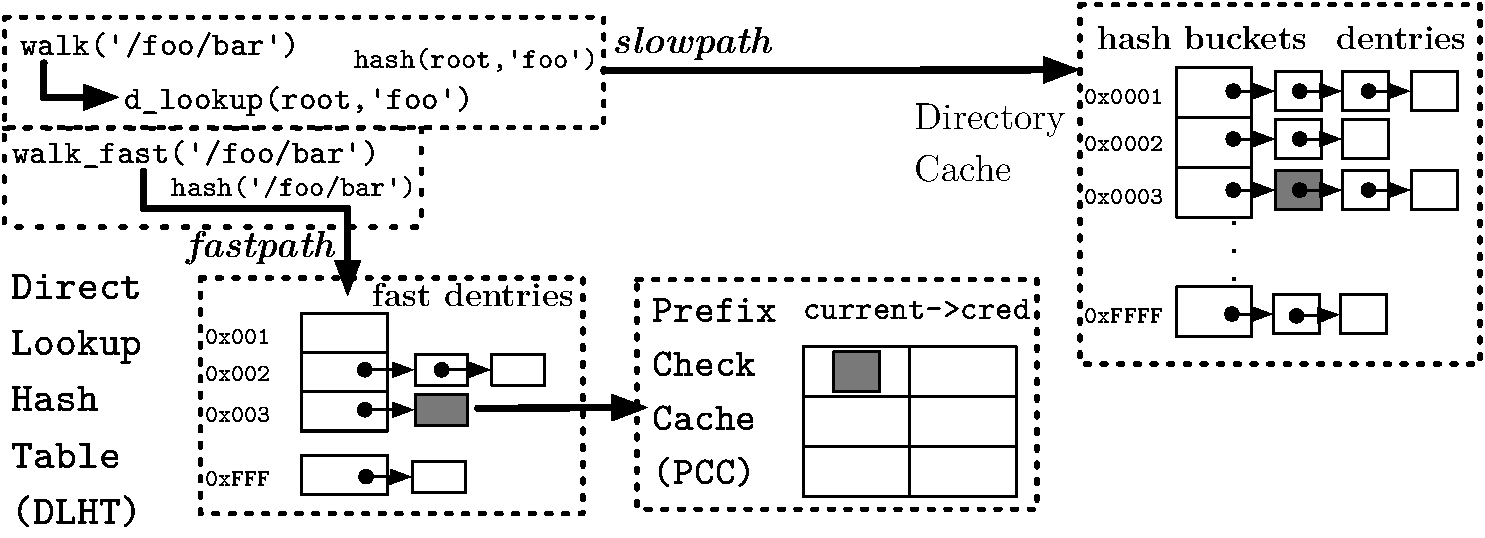
\includegraphics[width=4in]{dcache/figures/dcache-structure.pdf}
\footnotesize
\caption[Optimized Linux Directory Cache Structure.]
{Optimized Linux Directory Cache Structure. \dentries{} are chained in hash buckets. To index the hash bucket for a target \dentry{}, the original lookup routine {\tt d\_lookup} uses a hashing function with key as a combination of the pointer to parent directory and file name ({\em slowpath}).
Our {\em fastpath} hashes the full canonical path of target file to look up the \dentry{}
in the Direct Lookup Hash Table,
and checks the per-credential Prefix Check Cache.}
\label{fig:dcache}
\end{figure}

%\fixmedp{update the picture with new tables}
Like many Unix variants, Linux stores cached path-to-inode mappings (\dentries{}) in a hash
table (\S\ref{sec:background:dcache}).  This hash table is keyed by a combination of 
the virtual address of the parent \dentry{} and the next path component string, illustrated in
Figure~\ref{fig:dcache}.  
Virtual addresses of kernel objects do not change over time and are identical across processes.
%Each path component is checked for search permission in a top-down fashion,
%which we call a {\bf prefix check}.
%For instance, to look up component {\tt alice} in {\tt /home/alice/foo.txt},
%the kernel would take the virtual address of the \dentry{} for {\tt /home}, 
%and hash it with the string ``alice'' in order to find the bucket to search
%for the \dentry{} mapping ``alice'' to an inode, in order to check search permission on 
%the {\tt alice} directory.
%The latency of a prefix check, and thus a lookup, 
%grows linearly with the number of path components in the prefix.

In practice, prefix checks have a high degree of spatial and temporal locality,
and are highly suitable for caching,
even if this 
means pushing some additional work onto infrequent modifications of the directory structure (e.g., {\tt rename} of a directory).
RCU already makes this trade-off (\S\ref{sec:background:dcache}).

%Application file access patterns exhibit substantial temporal and spatial locality.
%Moreover, lookups (i.e., reads of the directory hierarchy)
%are vastly more common than modifications of the directory structure (e.g., {\tt rename} of a 
%non-empty directory) or permission changes within the directory structure (e.g., {\tt chmod} or {\tt chown} of a directory).


%% dp: Maybe cut this. Kind of meh
%% Caching prefix checks is analogous to caching access permissions along with 
%% virtual-to-physical translations in a hardware 
%% translation lookaside buffer (TLB). 
%% For instance, each level of an x86 page table encodes access permissions 
%% (e.g., read, write, execute, and user/kernel).  As the hierarchy grows deeper with larger address spaces
%% and hardware virtualization support~\citep{intel10, nestedpagetables}, 
%% needless loads can be elided.

%Linux's use of RCU already makes this trade-off (\S\ref{sec:background:dcache}).

In order to cache prefix check results, we must first decouple 
{\em finding} a \dentry{} from the prefix check.
We added a second, system-wide hash table exclusively for finding a \dentry{}, called the {\bf direct lookup hash table (DLHT)}.
%which only stores recently-accessed \dentries{},
%of \fixmedp{directories?}
The DLHT stores recently-accessed \dentries{}
hashed
by the full, canonicalized path.
A \dentry{} always exists in the primary hash table as usual,
and may exist in the DLHT.
The DLHT is lazily populated, and entries can be removed for coherence
with directory tree modifications (\S\ref{sec:dcache:rename}).

\begin{comment}
\fixmedp{proposed change; measure impact}
\fixmetsai{no done yet, and not sure about the impact. In general, if a file (a leaf) is constantly accessed, there is benefit to add it to DLHT.
Also a dentry found on fastpath means all of its ancestors have passed prefix checks, so if only directories stored, we still have to do one more check.}
%We limit the DLHT to directories because only directories 
%can be in a prefix.  Our lookup algorithm always does a second hashtable
%lookup in the primary hashtable for the final path component.
\end{comment}

Each process caches the result of previous prefix checks
in a {\bf prefix check cache} (PCC), associated with the process's credentials
(discussed further in \S\ref{sec:dcache:cred}), which can be shared among processes
with identical permissions.
The PCC is a hash table that caches dentry virtual addresses 
and a version number (sequence lock), used to detect stale entries (\S\ref{sec:dcache:rename}).
When a prefix check passes, indicating that the credentials are allowed to access the \dentry{}, 
an entry is added to the PCC; entries are replaced according to an LRU policy.
A miss in the PCC can indicate a permission denied
or 
%, which we believe is an uncommon case, or, more commonly,
that the permission check has not executed recently.

%The PCC is a hash table to quickly check if a dentry{} is recently prefix-checked.
%% dp: Meh
\begin{comment}
For simplicity, we implemented a set associative cache, resembling the design of a L1 cache in CPU, but a more sophisticated data structure such as
{\em Cuckoo hashing}~\citep{cuckoo04} can be even more efficient. 
\end{comment}
%lookup and insertion time asymptotically constant.
%The PCC is initially 64 entries, and in our current prototype doubles in size, up to a configurable
%maximum size,
%each time it exceeds a 50\% load factor.  
%If the maximum size and load factor are exceeded
%\fixmedp{implement}  





%% We changed the kernel path hashing strategy to 
%% simply hash the entire canonicalized path, rather than hash 
%% the virtual address of the parent \dentry{} and the next path component.
%% Thus, given any path, the kernel can directly look up the \dentry{} 
%% without walking the entire directory hierarchy.

%% We create a separate hash table, which we call a {\bf direct lookup hash table (DLHT)}.
%% When a \dentry{} is being hashed,
%% it is inserted into both \dcache{} hash table and fast lookup hash table,
%% using their hashing functions respectively.


%% Our {\bf first design} includes placing a {\bf prefix check cache (PCC)} into each \dentry{},
%% %which stores the results of up to \prefixcheckcachesize{} prefix checks,
%% %for \prefixcheckcachesize{} credentials who have most recently look up the \dentry{}.
%% which stores limited amount of prefix checks for credentials who have most recently looked it up.
%% Each cached prefix check is stored using one 64-bit word: 63 bits for a credential identifier
%% and one bit for the prefix check result.
%% However, adding prefix check cache largely increases the size of each \dentry{},
%% thus it will compress the total number of \dentries{} that can be loaded into RAM.
%% The prefix check caches in the most popular \dentries{}
%% will be frequently replaced
%% and have a high cache miss rate,
%% while the other ones can remain underused. 
%\fixmedp{If time, figure out how compact we can reasonably make this}
%The credential identifier, detailed in \S\ref{sec:dcache:selinux},
%represents the process's user id, group membership, capabilities, or any other credentials 
%that could have influenced the prefix check results.
%If any process attributes change that could influence a prefix check, the process must also change
%its credential identifier.


%% To improve space efficiency and cache miss rate of popular \dentries{},
%% our {\bf second design}
%% instead places a {\bf \dentry{} lookup table (DLT)}
%% into the Linux {\tt cred} structure (explained in section~\ref{sec:dcache:cred}).
%% The \dentry{} lookup table is a hash-based set-associative table,
%% and each of its entry contains two 32-bit words:
%% one for storing the lower 9th-40th bit of \dentry{} pointer that has been prefix-checked,
%% and the other for caching the sequence counter of the \dentry{} to determine whether it has been updated.
%% %(0 represents the prefix check has failed).
%% For each credential
%% we initially allocate a DLT with \lookuptablesize{} entries split in \lookuptableway{} ways.
%% The table can be dynamically extended if a credential is looking up more \dentries{},
%% and needs to cache more prefix check results. 

%% dp: worth exploring...
\begin{comment}
Thus, given any path prefix, the kernel
has a {\em fastpath} that directly looks up the prefix 
in the DLHT.  The fastpath case looks up the immediate
parent in the DLHT, checks cached permission for the entire prefix 
(described next), and then looks up the file itself in the primary hashtable.
If the fastpath fails, the code falls back on the original Linux lookup algorithm,
using the primary hashtable exclusively, and traversing components one at a time.
\end{comment}

Thus, given any path, the kernel
has a {\em fastpath} that directly looks up the path
in the DLHT.
If the fastpath hits in the DLHT,
the \dentry{} is then looked up in the process's PCC.
If a PCC entry is found and the version counter matches 
the cached counter, the cached prefix check result is used.
%with the same pointer is found and the sequence counter matches with the the \dentry{}, the results of the cached prefix check are used.
If the fastpath lookup misses in the DLHT or PCC, 
or the version counter in the PCC entry is older than the \dentry{}, 
the code falls back on the original 
Linux lookup algorithm (the {\em slowpath}),
using the primary hashtable exclusively and traversing one component at a time.

%\fixmedp{Chia-che, check this}
In the case of a relative path, such as {\tt foo/bar} under directory {\tt /home/alice},
we effectively concatenate the relative path and the path of the current working directory.
To implement relative paths, Linux already stores 
a pointer to the {\tt dentry} of the current working directory
in each process descriptor ({\tt task\_struct}).
Rather than {\tt memcpy} the strings, we store the intermediate state of the hash function 
in each {\tt dentry} so that hashing can resume from any prefix.

%\fixmedp{Chia-che check this; we should handle these cases; hacks are ok}
%\fixmetsai{revisited}
The current design includes two very infrequent edge cases.
First, a \dentry{} could be freed and reallocated with stale PCC entries.
We detect this case by initializing newly allocated \dentries{} with
%the maximum version number,
a monotonically increasing version number,
allowing PCC entries to detect staleness across reallocation.
Freeing a \dentry{} removes it from the DLHT.
Second, a version number can wrap around after every $2^{32}$ initializations of new dentries or
renames, chmods, or chowns
of non-empty directories; 
our design currently handles wrap-around by invalidating all active PCCs.
%entries less than $2^{31}$
%our design uses a garbage collector to scan all existing PCCs to gradually eliminate stale entries. \fixmetsai{need to implement}

\begin{figure}[t!]
\centering
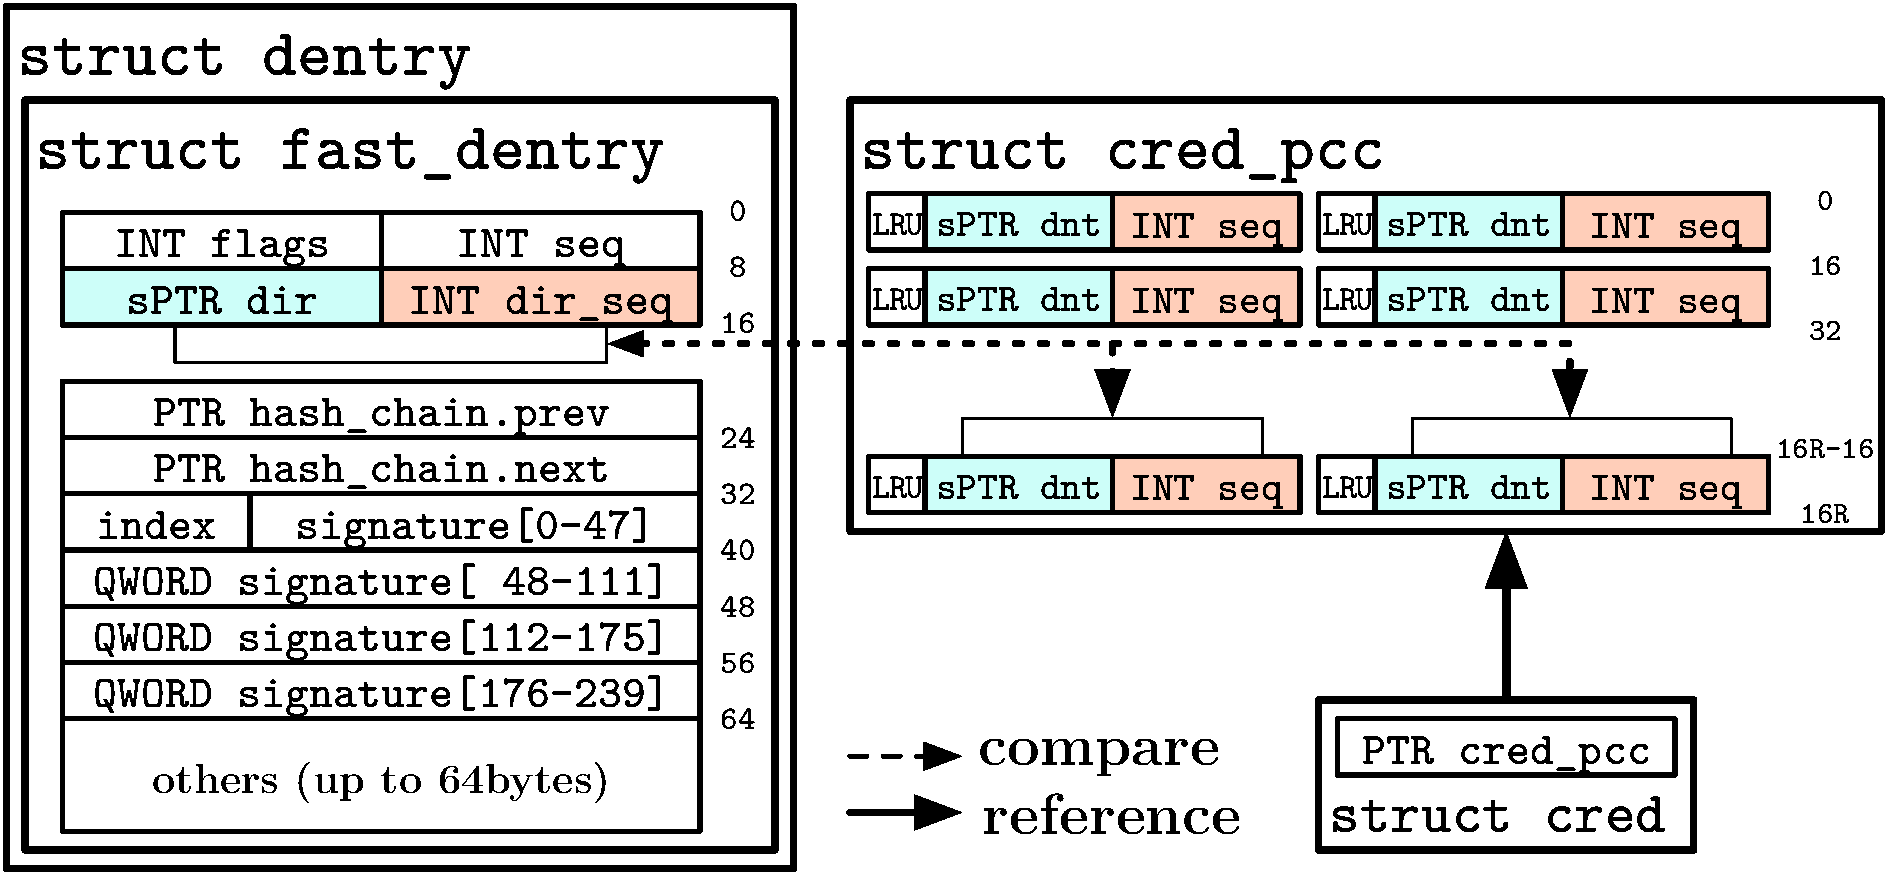
\includegraphics[width=4.5in]{dcache/figures/dcache-data_structure.pdf}
\footnotesize
\caption[Directory cache optimization: Data structures added.]
{Data structures added for fast directory cache lookup. To support {\em fastpath} lookup, we add a 88-byte fast dentry structure to the original \dentry{} and a variable-sized PCC structure into {\tt cred}. 
%% dp: meh
%Both structures are aligned to 64-byte cacheline to make lookup cache-friendly.
}
\label{fig:dcache-data-structure}
\end{figure}

Figure~\ref{fig:dcache-data-structure} illustrates the modifications 
to the Linux \dentry{} structure.  The {\tt fast\_dentry}
stores the signature, flags, a sequence count, a mount point,
lists for managing deep directory entries (\S\ref{sec:readdir:deep}),
and a list ({\tt hash\_chain}) for adding the fast\_dentry to a DLHT bucket.
The PCC is added to the kernel credential structure ({\tt struct cred}), %discussed in \S\ref{sec:dcache:cred}),
and stores a tunable number of tuples of \dentry{} pointers and sequence numbers;
the system is evaluated with a PCC of \PCCsize{}.
Because the highest and lowest bits in each \dentry{} pointer are identical,
the PCC only stores the unique pointer bits (8--39 in x86\_64 Linux) to save space.

%% SOSP Space
%% Although caching prefix checks is straightforward as described thus far,
%% this change 
%% causes ripples through the rest of the code, creating several additional challenges, such as 
%% keeping the cache coherent with modifications.
%% The following subsections address these challenges in the course of 
%% explaining the implementation in more detail.

%\fixmedp{Should we talk about signatures here? I'm tempted to push this to another subsection.}
%\fixmedp{Later: Make sure we explain how we shoot down entries somewhere}

% Order of subsections:
%% Credential IDs and generalization
%% Shootdown
%% Signatures and collisions
%% Special cases



%% \fixmedp{Move down...}
%% Permission caching is a simpler approach to determine file permission
%% than merging access rights of all parent directories.
%% The merging approach is used by related works like DLFS~\citep{lensing13dlfs},
%% which can only resolve permission based on
%% credentials of users and groups.
%% It cannot support more sophisticated access,
%% such as SELinux or AppArmor.
%% On the other hand, The permission caching approach requires no effort of
%% implementing permission merging,
%% thus it is able to support any access control,
%% including SELinux and AppArmor.
%% More details of access control support is discussed in section~\ref{sec:dcache:selinux}.

%% Using permission caching, our lookup method can calculate access right of
%% entering all parent directories to access target file,
%% without any sophisticated merging logic.
%% For every security credential, the access right is calculated by forcing
%% the lookup routine to fall back to the slow path at the first access on any file.
%% Because the slow path shares the exactly same logic as the original component-based lookup in Linux kernel,
%% it can rely on the existing routine of access right checking to determine permissions. 
%% This section will discuss more details about permission caching for fast directory cache lookup.

\subsection{Coherence with Permission and Path Changes}
\label{sec:dcache:rename}

When permissions on a directory or the directory structure are changed, such as with {\tt chmod} or {\tt rename},
any cached prefix checks that include this directory must be invalidated.
Our design  ensures the safety of concurrent lookups and changes by 
invalidating relevant PCC and DLHT entries before a change to the hierarchy,
preventing stale slowpath lookups from being re-cached, and leveraging VFS-level synchronization
to ensure correct slowpath behavior.
  
First, we ensure that a fastpath lookup cannot complete with stale data after a change to the directory structure.
Before a mutation, such as a {\tt rename} or {\tt chmod}, the operation 
must recursively walk all children in the \dcache{} 
and increment the {\tt fast\_dentry} version counter ({\tt seq}). % (steps a1--a4).  
The {\tt fast\_dentry} version counter is used by each process's PCC to detect changes to cached prefix checks on a lookup; % (step b2);
incrementing this version counter invalidates all PCC entries for that \dentry{} without directly modifying
each PCC.  
Changes to the directory structure (e.g., {\tt mount} and {\tt rename}) 
also remove \dentries{} under the old and new path 
from the direct
lookup hash table (DLHT).
PCC and DLHT entries are lazily repopulated on the slowpath.
%These paths can be lazily added back to the DLHT on the slowpath.

Second, we ensure that the results of a  stale slowpath lookup cannot be re-added to the DLHT or PCC by using an atomic, global sequence counter ({\tt invalidation}).
The sequence counter is read before and after a slowpath traversal; results are added to the DLHT and PCC only 
if the counter has not changed, implying no concurrent shootdowns.

Third, we use VFS-level synchronization to ensure that slowpaths synchronize correctly 
with the mutation. 
As an example, {\tt rename}
%%Before the rename begins, our code acquires the 
%%  {\tt invalidation\_lock}, invalidates the relevant children, 
%% acquires the appropriate 
%% VFS-level locks, and then releases the {\tt invalidation\_lock}.
%Rename has stricter requirements to ensure atomicity.
%In the case of {\tt rename}, 
acquires both
a global {\tt rename\_lock} sequence lock, along with per-\dentry{}
locks on the old and new parent directory.
When the {\tt rename\_lock} is held for writing, all lookups on the slowpath 
(i.e., the current Linux code)
must lock each \dentry{}
in a hand-over-hand fashion from the root (or current working directory, for relative paths) 
to the target child.
The locks on target \dentries{} obstruct the hand-over-hand traversal until the rename completes.
The {\tt invalidation} counter prevents caching the results of slowpath lookups that already passed 
this point before the \dentry{} locks were acquired.
%The {\tt rename\_lock} is held until all relevant DLHT entries are evicted,
%and our fastpath traversal is also retried if a concurrent rename is detected by the {\tt rename\_lock}'s sequence count.
%In the current Linux VFS, and our {\em slowpath}, 
Our implementation follows the VFS's existing locking discipline to avoid deadlocks;
it adds version counters that detect inconsistencies and falls back on the slowpath.
Thus, 
relevant PCC and DLHT entries are invalidated before the rename begins, blocking the fastpath;
slowpath traversals will block until the rename is complete
and the per-\dentry{} locks are released;
and a sequence counter ensures that only slowpath traversals that observe the new paths can repopulate the DLHT and PCC.



%% SOSP Space
%% Our \dcache{} design deliberately pushes some additional work onto the uncommon cases of 
%% directory permission changes or changes to the directory structure itself, in order
%% to accelerate frequent lookups.

%% dp: SOSP Space cut
%This is illustrated in Figure~\ref{fig:invalidation}.
%In order to invalidate PCC entries that refer to this directory's children, 
%a permission change operation 
%this choice avoids computing and updating
%prefix checks that will not be used.

%% dp: SOSP Space cut
%% Michael finds this hard to follow
\begin{comment}
\begin{figure}[t!]
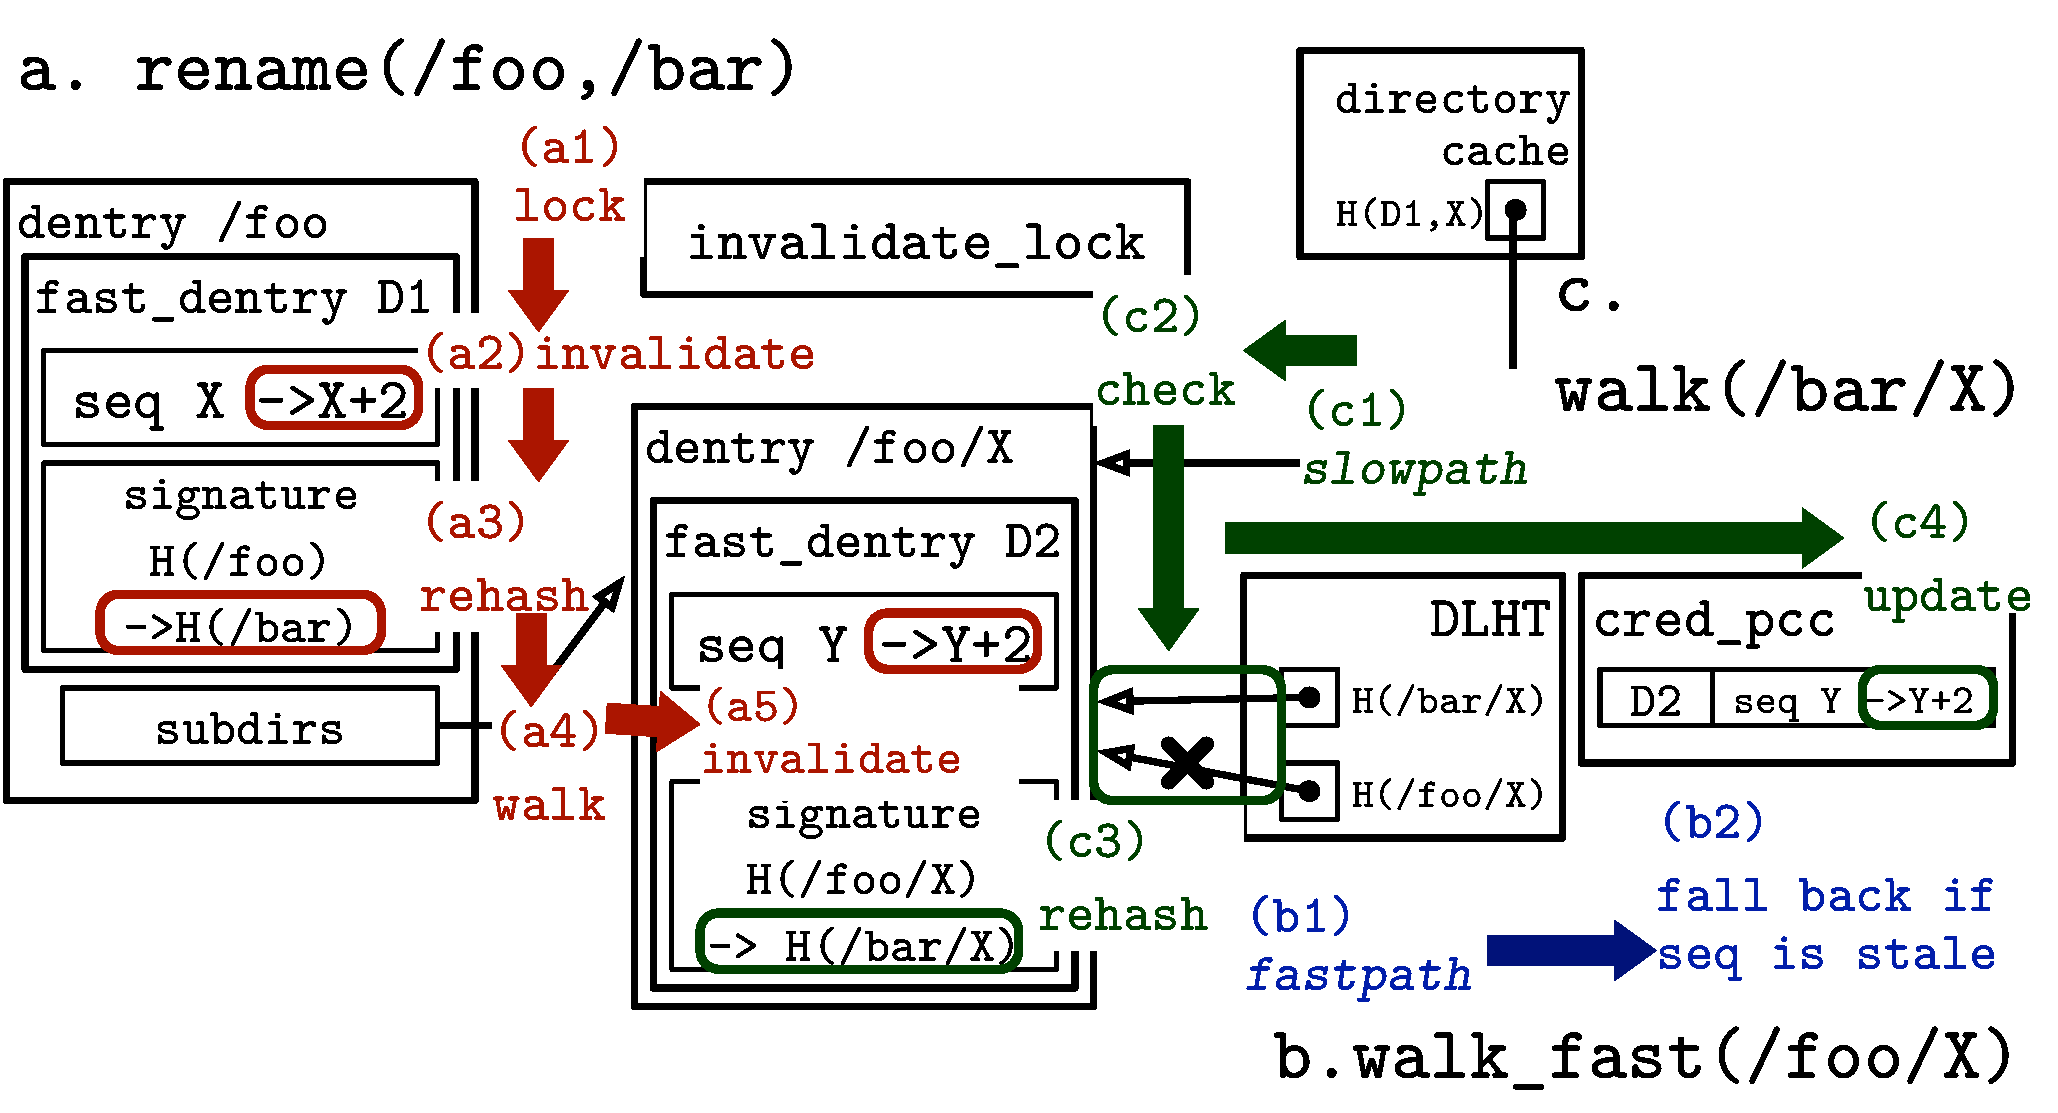
\includegraphics[width=1.0\linewidth]{dcache/figures/invalidation.pdf}
\vspace{-15pt}
\footnotesize
\caption{Procedure of updating directory trees for {\tt rename}/{\tt chmod} system calls.
The procedure {\color{red} (a)} invalidates the \dentries{} in all PCCs by incrementing the sequence counters {\color{red} (a2)}. The path will be rehashed. {\color{red} (a2)}.
The procedure then walks all child \dentries{} {\color{red} (a4)} and invalidate them {\color{red} (a4)} (but no rehashing).
A global lock will be held for coherence {\color{red} (a1)}.
If later the old path is looked up on the {\em fastpath} {\color{blue} (b)}, the found \dentry{} {\color{blue} (b1)} has a different sequence counter with the current PCC {\color{blue} (b2)}, thus revalidation is needed.
The forced {\em slowpath} {\color{OliveGreen} (c)} will look up the new path hierachically {\color{OliveGreen} (c1)}, check if the global lock is held {\color{OliveGreen} (c2)}, rehash signature {\color{OliveGreen} (c3)} and finally update the PCC {\color{OliveGreen} (c4)}.  }
\label{fig:invalidation}
%\vspace{-10pt}
\end{figure}
\end{comment}

%% Permissions changes are kept coherent  by 
%% causing fastpath traversals to retry on the slowpath when relevant \dentries{} change.
%% Slowpath traversals will always see a correct
%% view of the directory hierarchy via standard VFS-level synchronization.
%% Once a permission change is applied to a directory, the child version numbers are incremented
%% recursively.  
%% Once these changes are applied, any fastpath lookup will notice the difference in version numbers
%% between the child \dentry{} and the PCC entry, and retry the prefix check.

%% There is a brief window between the permission change of a parent and the version number change to a child.
%% A fastpath traversal during this time is equivalent to executing just before the permission change, which we consider acceptable, as no additional permissions can be acquired
%% and this window is quite short.
%% Similarly, a slowpath lookup  can start before the permission change, 
%% see the old value, and complete just after a permission change.
%% We prevent slowpath lookups from recreating potentially stale PCC entries
%% values by using a global sequence lock ({\tt invalidation\_lock}).



%We also increment the version counter on all children {\em before}
%the rename begins, and hold the
%Once a path is evicted from the DLHT, it 


%% dp: I think this is false
%A positive externality of this design is that the fastpath is never blocked by the {\tt rename\_lock} while {\em slowpath} can be forced to retry.  



\begin{comment}
\fixmedp{moved down from above (too early); dumped para here for now}
When directory structure changes, new prefix check result must be merged
onto every \dentry{} in the directory.
%In order to minimize the penalty on modifications,
We choose to lazily update the prefix check results, by preserving the original
component-based lookup algorithm as a fallback
while we temporarily block directly looking up the \dentries{} until the next access.


In the case of operations that influence a potentially-cached prefix check,
namely {\tt rename}, {\tt chmod}, {\tt chown},
and changes to security-relevant extended attributes,
we must clear the cached prefix check results on all descendants.
The way to clear cached prefix checks (or``to invalidate")
without actually zeroing any structures
is to force aging the sequence counters in the \dentries{}.
Specifically for {\tt rename}, we must also rehash all descendants in direct lookup hash table, because their canonical paths will also change.
\end{comment}

These recursive traversals shift directory permission and structure changes 
from constant time to linear in the size of the sub-tree.
As one example, 
%We found a simple recursive of the subtree to invalidate or rehash all descendants
%can be expensive in a deep directory.
 to {\tt rename} or {\tt chmod} a directory that has
10,000 descendants with at most depth of 4
takes roughly 330 microseconds to complete. 
%\fixmedp{updated numbers}
In the original Linux kernel, {\tt rename} and {\tt chmod} are nearly constant-time operations, and only take 4.5 and 1.1 microseconds.
A few applications, such as {\tt aptitude} or {\tt rsync},
rely on {\tt rename} to atomically replace a directory, 
but this is a small fraction of their total work % done even by these applications,
and orders of magnitude less frequent than lookups, making this a good trade-off overall.

\begin{comment}
The performance penalty for \fixmedp{app example} is \fixmedp{XX\%}.
\S\ref{sec:eval} includes more detailed measurements of these costs and the benefits of constant time lookup, indicating 
that this cost is acceptable.
\end{comment}
%We found a simple recursive walk of the subtree sufficient for our implementation, adding 12--16\% overhead 
%to {\tt chmod} of a directory---a very infrequent operation.
%To serialize readers, we hold the the parent dentry lock on the modified directory,
%which blocks the lookup slowpath until the modification is complete.
%Fast-path lookups which observe the old cached permissions are essentially serialized before the permission change.
%Subsequent executions of the slowpath will repopulate these caches.

\paragraph{Directory References.}
%\fixmedp{Chia-che check}
Unix semantics allow one to {\tt cd} into a directory, and continue
working in that directory after a subsequent permission change 
would otherwise prohibit further accesses.
%hold a reference to a file or directory
%after a permission check that 
%with an opened handle or the current working directory.
For instance, suppose a process is in working directory {\tt /foo/bar}
and {\tt foo}'s permissions change such that the process would not
be able to enter {\tt bar} in the future.
The process should be able continue to open files under {\tt bar}
as long as the process does not leave the directory or exit.
Similar semantics apply to open directory handles.
%Our solution must handle this use case without overriding the premission change.
%\fixmetsai{Don, I rewrote this part to reflect the current design. See if it make sense.}
In our design, such a permission change would ultimately result in a blocked PCC entry,
and a fastpath lookup would violate the expected behavior.
Our design maintains compatibility by
checking if the open reference is still permitted in the PCC.
If the PCC has a more recent entry that would prevent re-opening this handle,
the lookup is forced to take the 
the slowpath, and this stale result is not added to the PCC.

%If a PCC entry for {\tt /foo/bar} is inserted after {\tt /foo}'s permission change, future access to {\tt /foo/bar} will be allowed even after leaving or closing {\tt /foo}.
%This idiosyncrasy of isolating a working directory is supported by 

%If PCC no longer permits the current working directory or base handle, user can still look up paths inside the directory using 
 
%Our current prototype supports this idiosyncrasy by storing the version number
%of the current working directory as of the last {\tt cd};
%if the PCC entry is potentially newer, we only allow the slowpath 
%until the next {\tt cd}, for backward compatibility.
%We believe this is a case where the implementation has leaked into the interface,
%and a reasonable alternative in this situation would be to return an error, such as a stale file handle.

%% \paragraph{Updating Permissions.}
%% Access right of reaching a directory entry is determined by cached permissions
%% calculated in the slow path.
%% When the permission of a directory changes,
%% the kernel must invalidate all prefix check cache in every directory entry under the tree rooted at the directory,
%% to guarantee upcoming access to one of the directory entries be forced to
%% fall back to the slow path for recalculating the permission.

%% Invalidating of prefix check caches is required in two conditions:
%% \begin{compactitem}
%% \item Access permission of a directory is changed by {\tt chmod}, {\tt chown} or other system calls.
%% \item A directory is moved under a different parent directory.
%% \end{compactitem}
%% When invalidation is necessary, the kernel will traverse the whole tree of \dentries{} under the target directory,
%% and mark all \dentries{} as {\tt DENTRY\_INVALIDATED}.
%% If the {\em fastpath} finds a marked \dentry{}, it will fall back to component-based lookup,
%% which flushes the prefix check caches, unmark the \dentry{}, and revalidate the access permission. 

\begin{comment}
In order to mitigate the overhead on {\tt rename}, we push the work of rehashing onto the slowpath.
Because {\tt rename} also clears cached prefix checks,
any following lookup of the descendants
will be forced to fall back to hierarchical slowpath,
which can update direct lookup hash table complimentary.

Because we only invalidate \dentries{} at the operations like {\tt rename} and {\tt chmod}, and force consequential lookup to fall back to slowpath,
consistency of the directory structure is always maintained even if the operations happen concurrently.
The only exception is when a slowpath walk starts before a recursive invalidation happens,
and update a \dentry{} using wrong prefix check after it is invalidated,
the newly cached result will be counted as valid.
To prevent this scenario, we use a
global {\tt invalidate\_lock} sequence lock
to block prefix check caching
whenever an invalidation is in action.
This design is similar to the {\tt rename\_lock} used in the Linux kernel.

%\fixmedp{I see mount/umount as a case of shooting down entries.  I think the text below should be 
%merged in with rename discussion (although there are two sorts of shootdown)}
%\fixmetsai{The two kinds of shootdown is fundamentally different, because invalidation is to force lookup to fall back, but disconnection is to skip dentries while looking up.}

%Because dentries in our prototype are hashed by full path, rather than their parent pointer and file name,
%we must also recursively rehash all children and clear the prefix check cache when a 
%directory is moved.
%We find that this recursive traversal only increases the cost of a {\tt rename} by about 1\%.
% under a different directory.
%\fixmedp{Revisit if we save S4}

Because recursive invalidation can still be an major latency issue on some systems,
we provide an optimization to hide the overhead in the background
and remove penalty on the latency of operations that needs recursive invalidation.
The optimization use a kernel task to handle recursive invalidation
offline with spared CPU cycles.
The only caveat is that fastpath must be {\em disabled} when any invalidation is in process.

Finally, Unix specifies that when a file system is mounted over a non-empty directory,
all files or subdirectories under the directory will be disconnected from the system,
and become unavailable until the file system is unmounted.
We modify {\tt mount} to recursively invalidate all child \dentries{}.
When the file system is unmounted, these \dentries{} can be found again on slowpath and be resurrected for fast lookup.
\end{comment} 


%\paragraph{Disconnecting Directory Entries after Mounting.}
%Unix operating systems allow file system be mounted at any existing directories
%in the system.
%If the directory where mounting happens is not empty,

%In the original design, disconnecting \dentries{} is simple.
%Because all \dentries{} are looked up from their parents,
%disconnecting the root \dentry{} will automatically make all other \dentries{} in the tree unavailable.
%Our solution is to force a tree traversal to mark
%all \dentries{} under the tree as {\tt DENTRY\_DISCONNECTED}.


\subsection{Accelerating Lookups with Signatures}
\label{sec:dcache:collision}
\label{sec:dcache:signatures}

Our optimized lookup uses 240-bit signatures to minimize the cost of
key comparison.
Linux looks up \dentries{} in a hash table with chaining.
When the hash table key is a relatively short path component, the cost of simply 
comparing the keys is acceptable.  However, a full path on Linux can be up to 4,096 characters,
and comparing even modest-length strings can erode the algorithmic benefits of
direct lookup.
We avoid this cost by creating a signature of the path, which 
minimizes the cost of key comparisons.
%can 
%identify a path more compactly and 
%within a bucket of the direct lookup hash table.  

Using signatures introduces a risk of collisions, 
which could cause the system to map a path onto the wrong \dentry{}.
We first explain how signature collisions could cause problems in our design,
followed by the required collision resistance properties,
and, finally, how we selected the signature size to make this
risk vanishingly small.

%We use the multilinear~\citep{lemire2013strongly} 2-universal hash function to generate 192-bit signatures,
%a size selected to make the risk of a signature collision vanishingly small (analysis below).

%% Our fast lookup method uses a hashing function to map canonical paths of files
%% into indexes of hash buckets where the target directory entries are chained.
%% Because the number of hash buckets is limited,
%% collision will almost always happens.
%% In other word, two or more directory entries are often chained in the same hash bucket.
%% To correctly look up the files,
%% a collision detection method is necessary for differentiating directory
%% entries that matches the queried canonical paths.

%% We start with a naive solution of collision detection,
%% by store canonical paths in directory entries
%% and compare them against the queried paths during the lookup.
%% Although path comparison is always accurate
%% on differentiating directory entries,
%% storing canonical paths has expensive cost on memory space, and path comparison can significantly slows down the fast path.
%% The overhead of path storing and comparison may be smaller if the file system
%% has only very short paths,
%% but we cannot make any assumption of average path length in the system. 

%% A better solution of collision detection than path comparison
%% is to use a secondary hashing function to generate signatures of paths.
%% In this solution, each directory entry will have its signatures generated at allocation,
%% and stored inside the entry.
%% To look up a queried path, the lookup routine will map the path (canonicalized)
%% into the target signature
%% and compare it against directory entries in the hash bucket.
%% Because a signature is mostly shorter than the canonical path it represents,
%% storing and comparing it will have a lower overhead
%% on memory space and lookup time.

%%% dp: Although we are right to beat these guys up, I think it is a little too defensive
%%%     Let's save this for the rebuttal if needed
%% Unlike the path comparison solution, the signature-based solution can still cause
%% collision, but at a lower probability.
%% Although the signature-based (or hash-based) solution can be seen in several related work
%% such as DLFS~\citep{lensing13dlfs},
%% many of these works tend to underestimating the probability of collision.
%% Based on our verification, the system described in DLFS
%% actually have higher probability of collision than what the authors claim,
%% and cannot survive in systems that create millions of files. 
%% However, we prove that the signature-based solution can
%% actually be safe to use in our solution of file system directory cache lookup,
%% and the probability of signature collision is truly negligible.

%% dp: Let's start with the risks


\paragraph{Signature collisions.}
When a user looks up a path, our design first calculates a signature
of the canonicalized path, looks up the hash in the global DLHT,
and, if there is a hit in the DLHT, 
looks up the dentry and sequence number in the per-credential PCC.

A user can open the wrong file if the \dentry{} for another file 
with the same signature is already in the DLHT, and that \dentry{} is in the PCC.
For example, if Alice has opened file {\tt /home/alice/foo} with signature X,
and then opens file {\tt /home/alice/bar} that also has signature X,
her second open will actually create a handle to file {\tt foo}.
This creates the concern that a user might corrupt her own files through no fault of her own.  
%For instance, Alice might attempt to open a document for work and overwrite a photo she was just viewing.
This risk can be configured to be vanishingly small based on the signature size (discussed below).



Any incorrect lookup result must be a file that the process (or another process
with the same credentials) has permission to access.
For a fastpath lookup to return anything, a matching \dentry{} pointer must be in the task's PCC,
which is private to tasks with the same credentials.
Thus, a collision will not cause Alice to accidentally open completely irrelevant 
files that belong to Bob, which she could not otherwise access.

%\fixmetsai{Don, I am moving this paragraph here, since it looks like a direct follow-up to the previous paragraph.}
Our design correctly handles the case where 
two users access different files with the same signature,
because misses in the PCC will cause both users to fall back on the slowpath.
%Our design does best-effort collision detection when two users access different files
%with the same signature.
Suppose Bob has opened {\tt foo}, which collides with Alice's {\tt bar}.
When Alice opens {\tt bar}, its signature will 
match in the DLHT, but will miss in the PCC.
This causes Alice's lookup to take the slowpath
to re-execute the prefix check,
ultimately opening the correct file and adding this \dentry{} to her PCC.
%The prefix check will return a result and a pointer to the dentry 
%for {\tt bar}, which is added to Alice's PCC.
%Alice will use this cached \dentry{},
%pointing to the correct file ({\tt bar}), not Bob's {\tt foo}.
Thus, if Bob were adversarial, he cannot cause 
Alice to open the wrong file by changing dcache-internal state.
% experience a collision by influencing dcache state,
%except to lower it by evicting Alice's files from the DLHT.

We choose a random key at boot time for our signature hash function,
mitigating the risk of deterministic errors or offline collision generation,
as one might use to attack an application that opens a file based on user input, such as web server.
Thus, the same path will not generate the same signature 
across reboots or instances of the same kernel.
%Based on the expected success rate of a brute-force attack,
%explained below, one could also periodically drop the cache and rekey the signature function,
%although we expect this would only be needed in a system with years-to-decades of uptime and orders-of-magnitude more powerful hardware than current systems.

%% When signatures replace full path comparisons, the concern is that the 
%% kernel may open a different file than the one the user intended.
%% The worst case is when a user, Alice, looks up two different paths with colliding signatures,
%% both take the fast path, and the second lookup returns the first file.
%% In this case, Alice cannot open any files she couldn't otherwise access, but may open the wrong file.
%% %In the rare event this happens, all permission checks will execute correctly, 
%% %so the user cannot access any files she couldn't otherwise access.
%% Signature collisions are detected on the {\em slowpath},
%% which is always taken the first time a user accesses a given path; colliding paths are permanently blocked from the DLHT with a \dentry{} flag.
%% %\fixmedp{add collision detection?}
%% Thus, an adversarial user, Mallory, cannot influence 
%% the risk Alice will experience a collision,
%% except to lower it by evicting Alice's files from the DLHT.
%Finally,
%We mitigate the risk of 
%deterministic errors or offline collision generation 
%by %salting
%using a random key for our signature hash function chosen at boot time, keeping signatures
%hidden from users, and using a collision-resistant hash function (discussed in more detail below).

%% Thus, the one remaining and important concern about optimizing lookup with a signature comparison
%% is that a user might corrupt her own files through no fault of her own.  
%% For instance, Bob might attempt to open a document for work and overwrite a photo he was just viewing.
%% This risk is configurable based on the signature size.  

Despite all of these measures, 
this risk may still be unacceptable for applications running as root,
which can open any file,
especially those that accept input from an untrusted user.
For example, suppose a malicious user has identified
a path with the same signature as the password database.
This user  might pass this path to a setuid-root utility
and trick the setuid utility into overwriting 
the password database.
This risk could be eliminated by disallowing signature-based 
lookup acceleration for privileged binaries or security-sensitive path names,
although this is not implemented in our prototype.

% (generally \fixmedp{XX-YY (bill says 160--256, but no handy cites)} bits)\fixmedp{cites}.

%% Because this is unacceptable behavior, we select a signature such that
%% collisions will be indistinguishable from disk sector corruptions.
%% Although we do not do this in our prototype, 
%% even this risk could be eliminated for 
%% for root processes by using more expensive checks.

\paragraph{Collision Resistance Requirements.}
The security of our design hinges on an adversary only being able to find collisions
through brute force.  
Our design can use either a 2-universal hash function or a pseudorandom function family (PRF)
to generate path signatures.
%; the 
%principal concerns are performance and risk of side channels.
In terms of collision resistance, the difference between a 2-universal hash
and a PRF is that the adversary can potentially learn the secret key 
by observing the outputs of the 2-universal function, but cannot learn the key from 
the outputs of a PRF.
Because our dcache design does not reveal the signatures to the user,
only whether two paths have a signature collision,
a hash function from either family is sufficient.

One caveat is that, with a 2-universal hash function, 
one must be careful that timing and other side channels do not leak 
the signature.  For example, one cannot use bits from the signature
to also index the hash table, as one might learn bits of the signature from 
measuring time to walk the chain on a given hash bucket.
In the case of our selected function, one can safely use the lower bits from 
the 256-bit hash output, as lower bits are not influenced by the values in higher bits in our particular algorithm;
we thus use a 16 bit hash table index and a 240-bit signature.
In contrast, when the signature is generated with a PRF,
concerns about learning the signature from side channels are obviated.

Our design uses the 2-universal multilinear hash function~\citep{lemire2013strongly}.
%and we carefully audit any code that calculates or compares signatures for potential side channels.
We did several experiments using PRFs based on the AES-NI hardware, and could not
find a function that was fast enough to improve over baseline Linux.
% until  paths had 4 or more components. \fixmedp{Still true?}
Using current 128-bit AES hardware, we could improve performance at 4 or more path components,
but creating a 256-bit PRF required a more elaborate construction that is too expensive.
%This was largely because we could not get enough bits from the 128-bit AES hardware without adding more elaborate constructions.
A more cautious implementation might favor a PRF to avoid any risk of overlooked side channels, especially
if a fast, 256-bit PRF becomes available in future generations of hardware.


%% SOSP Space
\begin{comment}
\begin{figure}[t!]
\centering
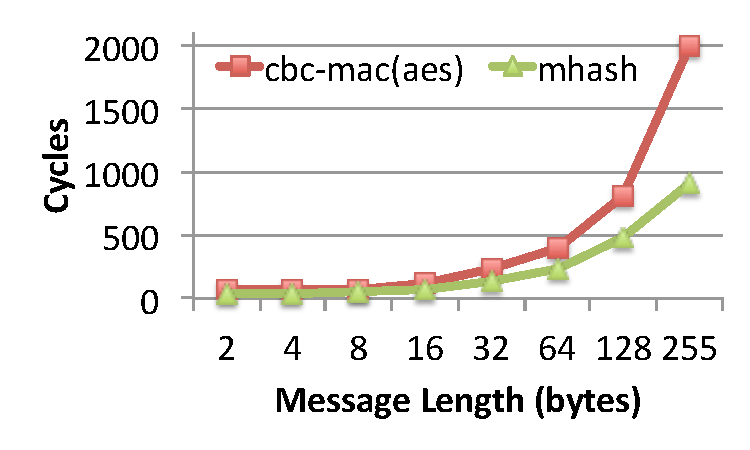
\includegraphics[width=.7\linewidth]{dcache/plots/hash.pdf}
\vspace{-10pt}
\footnotesize
\caption{
Cycles to hash messages of varying sizes using the 2-universal multilinear hash (mhash) and using the PRF cbc-mac(aes) using the Intel AES-NI instructions.
Lower is better; at lower values, cbc-mac(aes) is roughly twice as slow as mhash. }
\label{fig:hash}
\vspace{-10pt}
\end{figure}

Thus, the main reason to select a 2-universal function over a 
PRF is performance.  
Our design can use a hash function from either family.
Figure~\ref{fig:hash} compares the performance of hashing different message lengths
using the 2-universal multilinear hash function~\citep{lemire2013strongly}  (mhash)
and, as a PRF,
the CBC-MAC algorithm with hardware-accelerated AES
as the block cipher.
Because AES only creates a 128-bit hash value, we ran the algorithm twice with different keys to create a 256-bit output;
as a result, using CBC-MAC(aes) takes roughly twice as long as mhash.
In terms of the impact this has on lookup performance, 
mhash can outperform baseline Linux even for a single-component path,
whereas CBC-MAC(aes) is only faster than Linux with four path components.
We expect that, with hardware support for a 256-bit hash output, a PRF would be equally practical
for our purposes.

In order to realize the best performance, we use the mhash function in our experiments,
and carefully audit any code that calculates or compares signatures for potential side channels.
\fixmedp{Clear this fixme when done}
A more cautious implementation might favor a PRF to avoid any risk of overlooked side channels.
\end{comment}

%% \fixmedp{Educated speculation from here forward.  Revisit once we have numbers}
%% For a PRF, we used the CBC-MAC algorithm to create a signature, using AES
%% as the block cipher.  
%% Because AES only creates a 128-bit hash value, we ran the algorithm twice with different keys to create a 256-bit output.
%% In our experiments, hardware-accelerated AES instructions make the cbc-mac(aes)
%% fast enough to accelerate lookup by \fixmedp{XX\%} for the test in Figure~\ref{fig:by-version}.
%% The 
%% also improves lookup by \fixmedp{XX\%} in this test.
%% Because the improvements from a 2-universal hash are marginal,
%% we err on the side of caution and report only results with a PRF-based signature.


\paragraph{Probability of a signature collision.}
We selected a 240-bit signature, 
which is comparable to signature sizes used in data 
deduplication systems, ranging from 128--256 bits.  Deduplication designs commonly 
select a signature size that introduces a
risk of collisions substantially less than the risk of undetected ECC RAM 
errors~\citep{Debnath:2010:CSU:1855840.1855856, Srinivasan:2012:ILI:2208461.2208485, Quinlan:2002:VNA:645371.651321, Zhu:2008:ADB:1364813.1364831}.

We assume an adversary that is searching for collisions by brute force.
This adversary must lookup paths on the system,
such as by opening local files or querying paths on a web server.
Because our hash function is keyed with a random value and the output is 
hidden from the user,
the adversary cannot search for collisions except on the target system.
Thus, the adversary is limited by the rate of lookups on the system,
as well as the capacity of the target system to hold multiple signatures
in cache for comparison.

%Assuming an adversary is using brute force to find a collision,
We calculate the expected time 
at which the risk of a collision becomes non-negligible (i.e., higher than $2^{-128}$) 
%to find a collision 
%with a 240-bit hash value, and
%Suppose the adversary makes $t$ attempts to look up any paths in the directory cache, 
and model the risk of collision as follows.
First, $|H(X)|=2^{240}$ is
the number of possible signatures.
We  limit the cache to $n=2^{35}$ entries (i.e., assuming 10TB of dcache space in RAM and 320 bytes per entry),
with an LRU replacement policy.
We calculate the number of queries ($q$) after which the risk of a collision is 
higher than $P=2^{-128}$ as follows:
\begin{align*}
q \simeq ln(1 - p) * \frac{|H(x)|}{-n} \simeq ln(1-2^{-128}) * \frac{2^{240}}{-2^{35}} \simeq 2^{77}
\end{align*}
At a very generous 
lookup rate of 100 billion per second (current cores can
do roughly 3 million per second),
the expected time 
%in the brute force attack
at which the probability of a brute-force collision goes above $2^{-128}$
is 48 thousand years.

%% If one does a similar calculation with a completely unbounded 
%% dcache (i.e, each new signature is compared against all previous signatures),
%% the expected time drops to 8 years.
%% In such a worst case, the cache can be dropped and a new random signature key selected
%% after every 8 years of uptime, but with any reasonable bound on the cache size,
%% this should not be a concern.

%% and an uptime of 10 years, for $t \simeq 3.16 * 10^{19}$.
%% We assume an unbounded directory cache.
%% The probability of successfully causing any collision is:

%% \vspace{-0.15in}
%% \begin{align*}
%% P_{Adv}(t,H(X)) \simeq 1 - \epsilon^{-\frac{t^2}{2|H(X)|}}
%% \end{align*}
%% \vspace{-0.15in}

%% Thus, with 192 signature bits, the probability of a collision
%% is less than XXX, which is algorithmically negligible.

%% In order to less than a one in a billion \fixmedp{machines?}
%% the number of attempts by the adversary must be at least:

%% \vspace{-0.15in}
%% \begin{align*}
%% T_{Adv}({10}^{-9},2^{192}) \simeq \sqrtsign{\ln{(1-{10}^{-9})} \times -2 \times 2^{192}} \simeq 2^{81}
%% \end{align*}
%% \vspace{-0.15in}


%% In a system with 10-year uptime, assuming the directory cache is never shrinked, an adversary must perform at least ${10}^{17}$ lookups per second, to achieve one success in a billion manipulated systems. Such an adversary is computationally impossible to succeed in the real world.

%% \fixmedp{I'm confused.  We seem pretty far from $2^{-128}$.  Also, I'm not sure why we are talking about the number of systems.  Let's assume the number of systems is independent and focus on one system, since each has a different random key.}

\begin{comment}

\fixmedp{Chia-Che, please update these calculations.  What happens if we do things Michael's way?}
\fixmedp{once this is resolved, respond to D6}
\fixmedp{Add a note that this is an upper bound and why (just check that what is going on is clear after revision}

We consider two possible collision cases separately.
First, consider the case where two \dentries{} in the cache have a 
matching signature.
This type of collision could cause an application to access the wrong file,
and eventually retrieve wrong content or corrupt the file.
The probability of this type of collision is:
%
\begin{align*}
P_+(n,H(X)) = \frac{n(n-1)}{2} \times \frac{1}{|H(X)|} \simeq \frac{n^2}{2|H(X)|}
\end{align*}
%
where $n$ is the number of directory entries in the system, and $|H(X)|$ is
the number of possible signatures.  

The second type of collision happens if a user 
asks for a path that does not exist in the cache, which 
collides with an existing directory entry
with a different path.
This type of collision will cause the application to
assume existence of a nonexistent file and potentially corrupt other files.
The probability of this type of collision among $q$ queried paths is:

\vspace{-0.15in}
\begin{align*}
P_-(n,H(X),q) = 1 - (1 - \frac{n}{|H(X)|})^q \simeq 1 - \epsilon^{-q\frac{n}{|H(X)|}}
\end{align*}
\vspace{-0.15in}

We argue that the probability of both types of collision is negligible
when using a 192-bit universal hashing function to generate path signatures.
In our assumption, most systems will devote no more than 16GB of physical memory in directory cache, indicating that at most $\simeq 10^8$
\dentries{} will coexist at the same time.
A very busy system with a 10-year uptime, performing an average of 1000 lookup per second,
will query the directory cache for $3\times{10}^{11}$ times ($=q$).
%The number of directory entries is much smaller than
%the number of actual files and directories on storage because directory cache only keeps entries
%that are most recently accessed.
%has the longest possible history of queries.
Using a 192-bit signature, number of possible signatures is ${2}^{192}$ (=$|H(X)|$).
The probability of either collision can be calculated as follows:

\vspace{-0.15in}
\begin{align*}
P_+(10^8,{2}^{192}) \simeq \frac{{(10^8)}^2}{2\times{2}^{192}} \simeq {2}^{-139}
\end{align*}
\vspace{-0.28in}
\begin{align*}
P_-(10^8,{2}^{192},3\times{10}^{11}) \simeq 1 - \epsilon^{-3\times{10}^{11}\frac{10^8}{{2}^{192}}} \simeq {2}^{-128}
\end{align*}
\vspace{-0.15in}

In conclusion, with a directory cache no larger than 16GB, 192-bit signatures make the risk of collision 
negligible within $3\times{10}^{11}$ lookup operations,
or roughly every 10 years.
If a system decides to dedicate more physical memory than 16GB in directory cache,
longer signatures will have to be used,
or a shorter life span of the system must be assumed.
We can enforce this assumption and mitigate the risk of brute force attacks 
by changing the signature key,
and dropping or recalculating the signature for all dcache entries
after this threshold of lookups has been met.

\paragraph{Adversary Resistance.}



Because permission check only happens on the {\em slowpath}, signature collision will never cause security breach with benign users. However, many priviledged processes (e.g. Setuid-to-root programs, system services) in the system can be manipulated by a malicious user to exploit signature collision.
Fortunately, the strength of such an adversary is limited by the system latency, because it cannot perform an offline attack to the signature algorithm, but brute-forcely attempt for lookup in the system.

Assume a stronger adversary uses {\em Birthday Attack} to discover any pairs of paths that have signature collision. Suppose the adversary makes $t$ attempts to look up any paths in the directory cache, the probability of successfully causing any collision is:

\vspace{-0.15in}
\begin{align*}
P_{Adv}(t,H(X)) \simeq 1 - \epsilon^{-\frac{t^2}{2|H(X)|}}
\end{align*}
\vspace{-0.15in}

In other word, to achieve $10^{-9}$ success rate (one in a billion machines), the number of attempts by the adversary must be at least:

\vspace{-0.15in}
\begin{align*}
T_{Adv}({10}^{-9},2^{192}) \simeq \sqrtsign{\ln{(1-{10}^{-9})} \times -2 \times 2^{192}} \simeq 2^{81}
\end{align*}
\vspace{-0.15in}

In a system with 10-year uptime, assuming the directory cache is never shrinked, an adversary must perform at least ${10}^{17}$ lookups per second, to achieve one success in a billion manipulated systems. Such an adversary is computationally impossible to succeed in the real world.
\end{comment}



%The probability of either type of collision is lower than $2^{-128}$,
%which is algorithmically negligible.
%Because mean-time-to-failure (MTTF) of most hard drives ranges from $10^6$ to $1.5\times10^6$ hours~\citep{schroeder07mttf},
%any directory collisions will be indistinguishable from a disk sector 
%failure that corrupts directory metadata.
%\fixmedp{Let's consider dropping the first case for space here.}

%it is guaranteed that any systems will have to restart to recover from disk \fixmedp{sector?} failures before collision happens in the directory cache.

%At high probability, the collision will never appear in the history of queries
%before the system is restarted.

%% The only possible attack using signature collision is to maintain
%% an oracle of all queried paths for brute-force attack across system restart.
%% To defend this attack, we use a randomly generated seed to randomize
%% the hashing function every time the system starts. 

%% In our threat model, we are not defending any offline birthday attack
%% that deliberately queries two paths or creates two files that are known to
%% have colliding signatures.
%% These attacks is not a threat for us because they cannot bypass
%% permission check while accessing the files.
%% In most cases, an adversary that uses birthday attack can only corrupt
%% a file that it already owns the access right.
%% The worst scenarios is that the adversary may trick a seteuid-to-root
%% program to enter a directory which it does not have privilege to.  



\begin{comment}
A good design of caching systems requires a fully optimized lookup method,
which uses the fastest way possible to
determine whether requested data exists in the cache.
Efficiency of the lookup method is especially essential and dominating the
overall lookup performance when
the caching system has a significantly high hit rate.
In the directory cache, a high hit rate can be expected in file systems with temporal locality in file access pattern, low memory pressure
and infrequent metadata relocation.
We predict that these characteristics can be found in majority of systems,
because applications are inclined to access files repeatedly,
and enough spared memory is often available.
These systems will certainly benefit from any improvement on the efficiency of
directory cache lookup.

The directory cache in current Linux kernel uses component-based lookup.
To search for a requested file, the lookup routine will scan and delimit 
every component in path of the file,
and iterate through chained entries in correspondent hash buckets as many times
as the number of components.
The latency of directory cache lookup will grow linearly as longer and deeper
paths are queried.
Despite many efforts have been made in Linux kernel, directory cache lookup
is still one expensive cost to pay in many file system operations. 

We present the design of a significantly faster directory cache lookup
for Linux \linuxver{} kernel.
The lookup method can maximize the speed of searching
a directory entry for a target file which is previously accessed and 
has its metadata cached in memory.


The basic design of our lookup method is simple:
To search the directory entry for a requested file,
instead of breaking the path of file into components and iterates hash buckets repeatedly,
we use a hashing function that maps the whole canonical path of the file
into the index of hash bucket,
and directly look up the directory entry that stores the metadata of the last component.
If the directory entry is found, it is returned immediately to caller routine
for file system operations.
If the directory entry is not found, it is a case of cache miss.
When a cache miss happens, VFS asks file system drivers to locate
and retrieve metadata from the storage.
\end{comment}

%% To deal with cache misses,
%% our solution keeps the original component-based lookup method of Linux kernel,
%% as a slow path to fall back when our lookup method fails searching the
%% directory entry.
%% When a cache miss happen, even if the directory entry for the requested file
%% does not exists in the cache, the parent directories of the file may have been
%% accessed and have their directory entries created.
%% Using component-based lookup as slow path can recollect all created parent
%% directory entries, and request file system drivers to retrieve metadata of the rest
%% of parent directories and the files to cache.
%% Because the file system driver interface of Linux kernel is designed to look
%% up metadata by the parent directory and a file name,
%% using component-based lookup can keep file system drivers unchanged,
%% which can largely alleviate the pain of porting third-party file system driver
%% codes to the new directory cache design.

%% Another reason of using component-based lookup as slow path is to
%% calculate user access right against the target file.
%% To allow an user to access a file, the user requires not only the privileges
%% of file operations,
%% but also permission to enter every parent directory of the file.
%% The easiest way of calculating the permission is to resolve the access right
%% at each parent directory,
%% while looking up entries by each component of the path.
%% Once the permission of a directory or a file is calculated in the slow path,
%% we cache the permission in directory entry
%% and reuse it to determine the access right at next time when
%% the directory entry is looked up in the fast path.
 
%% The permission cached in directory entries is bound to the user credential
%% of process who performs the slow path.
%% If a different user credential look up a directory entry by the fast path,
%% it cannot be guaranteed to have permission to access the file.
%% For example, user {\tt A} and {\tt B} accesses the file {\tt /home/foo/bar},
%% but only user {\tt A} has the permission to entry the directory {\tt /home/foo}.
%% If user {\tt A} has accessed the file first, the kernel will create the directory
%% entry of {\tt /home/foo/bar}, which can be directly looked up in the fast path
%% by user {\tt B}.
%% In these cases of {\bf permission cache miss}, we must
%% force directory cache lookup to fall back to the slow path, in order to calculate
%% the access right for the new user credential.




%% The design of constructing a faster lookup method upon a slower one
%% is comparable to the concept of {\bf TLB (translation lookaside buffer)}.
%% TLB is a hardware optimization of multiple-level page tables traversal
%% in MMU to
%% translate virtual memory addresses into physical pages.
%% By falling back to page table traversal, TLB can recover from incoherence
%% without a sophisticated synchronization and update scheme.
%% The operating system only needs to flush the TLB timely whenever incoherence
%% is suspected or the page table needs to be updated.
%% Similarly, our fast lookup method for file system directory cache works without
%% any logic to update or to sync up directory entries, but simply fall backs to
%% slower component-based lookup to reassure coherence.

%% \paragraph{Expected Speed-up of Lookup Time}
%% Based on expected hit rate, we can predict the average lookup time
%% in directory cache
%% before and after applying the fast path:

%% \vspace{-0.22in}
%% \begin{flalign*}
%% & {Lookup\;time}_{original} = {Time}_{slow\;path} + {Time}_{storage\;lookup} \\
%% & \times (1 - (Hit\;rate))\\
%% & {Lookup\;time}_{optimized} = {Time}_{fast\;path} \times (Hit\;rate) \\
%% & + ({Time}_{slow\;path} + {Time}_{storage\;lookup}) \times (1 - (Hit\;rate))
%% \end{flalign*}
%% \vspace{-0.22in}

%% From the expected lookup times, we can calculate the improvement of performance as follows:

%% \vspace{-0.22in}
%% \begin{flalign*}
%% & {Speed\;up} = \frac{({Time}_{slow\;path} - {Time}_{fast\;path}) \times (Hit\;rate)}{{Lookup\;time}_{original}}
%% \end{flalign*}
%% \vspace{-0.22in}

\section{Generalizing the Fast Path}
\label{sec:generalize}

Thus far, we have explained our fast path optimization using the relatively straightforward
case of canonical path names.  
This section explains how these optimizations integrate with Linux's
advanced security modules,
%, such as SELinux~\citep{selinux} and AppArmor~\citep{apparmor},
as well as how we 
address a number of edge cases in Unix path semantics,
%which must be implemented correctly, 
such as mount options, mount aliases, and symbolic links.  
%Linux also includes a number of  which must work correctly with any VFS-level optimizations.
%This section explains how we address these challenges.

\subsection{Generalizing Credentials}
\label{sec:dcache:cred}
\label{sec:dcache:selinux}

%Two key requirements of our dcache optimizations are that they must be general
%and that space overheads for extra metadata must be minimized.
Linux includes an extensible security
module framework (LSMs~\citep{wright+lsm}), upon which SELinux~\citep{selinux}, AppArmor~\citep{apparmor}, and others are built.
An LSM can override the implementation of search permission checks,
checking customized attributes of the directory hierarchy or
process.
Thus, our dcache optimizations must still work correctly even when an LSM overrides the default access control rules.
%the default definition of 
%we need a general mechanism to encapsulate all possible credentials of a process with minimal 
%space overhead in the \dentries{}.

Our approach leverages the {\tt cred} structure in Linux, which is designed to store 
the credentials of a 
process ({\tt task\_struct}), and has several useful properties.
First, a {\tt cred} struct is comprehensive, including all variables that influence default permissions,
and including an opaque {\tt security} pointer for an LSM to store metadata.
Second, a {\tt cred} is copy-on-write (COW), so when a process changes its credentials, such as 
by executing a {\tt setuid} binary or changing roles in SELinux, 
the {\tt cred} is copied.  We manually checked 
that AppArmor and SELinux respect the COW conventions for changes to private metadata.
Moreover, a {\tt cred} can be shared by processes in common cases, such as a shell script forking children with the same credentials.
Thus, the {\tt cred} structure meets most of our needs, with a few changes, which we explain below.

%\fixmedp{Clarify per-process is shared with common cred}

%As explained in Section~\ref{sec:dcache:prefixcheck}, 
We store cached prefix checks (\S\ref{sec:dcache:prefixcheck}) in each  {\tt cred} structure,
coupling prefix check results with immutable credentials.
New {\tt cred} structures are initialized with an empty PCC.
When more processes share the PCC, they can further reduce the number of slowpath lookups.


%% describe two designs of prefix check caching:
%% one is using a prefix check cache in each \dentry{},
%% and one is using a \dentry{} lookup table in each {\tt cred} structure.
%% The former uses a 63-bit integer, called the credential identifier (CID), as a layer of indirection to {\tt cred},
%% while the latter simply places a pointer in {\tt cred} to reference the DLT.
%% Using CID, we must handle the very infrequent case of CID wrap-around.
%% Using DLT, we can avoid handling CID wrap-around, and have better space efficiency as explained in section~\ref{sec:dcache:prefixcheck}.

%to minimize the complexity of freeing and reallocating the {\tt cred} structure itself.
%A simple alternative would have been to simply store the kernel virtual address of the {\tt cred} in 
%various \dentry{} prefix caches, but these caches would have to be cleared before the {\tt cred} is 
%freed, lest a recycled {\tt cred} obtain access to a stale prefix.
%Rather than incur this bookkeeping cost, we simply assign a unique CID integer value to 
%Each time a {\tt cred} is allocated and reused, a new CID is assigned to the cred.
%The CID approach allows stale CID's to safely persist in a prefix cache until they are evicted by LRU,
%and does not complicate freeing a {\tt cred}.

%Using CID, we must handle the very infrequent case of CID wrap-around
%by simply resetting 
%the CID of all active {\tt cred} and clearing all prefix caches.
%We note that, even if an extremely efficient machine changed credentials one trillion 
%times per second
%(cf.\ current cores process at most 4 billion instructions/second),
%a wrap-around would occur once every 106 days. 
%We believe this is acceptable:
%most end-user machines reboot for kernel patches more frequently than this, 
%and even highly-available systems can afford to clear the prefix check cache 
%(not the entire dcache) a few times a year in exchange for the demonstrated benefits.



% reuse
%% The key challenge of implementing permission caching is
%% to identify security credentials within cached permission records in each directory entry.
%% If the access rights of a process are changed, such as updating user/group ID by calling system call {\tt setuid} and {\tt setgid}, or applying new SELinux labels or AppArmor rules,
%% the previous cached permissions should not be
%% reused in the lookup routine if it can cause privilege escalation.

%% Our solution uses the {\tt cred} structure defined in Linux kernel to identify different security credentials.
%% The {\tt cred} structure is a kernel structure referenced by {\tt task\_struct},
%% to store all real/effective user/group IDs, capability, security labels and security records of processes.
%% The {\tt cred} structure can be shared by related threads and processes,
%% so child processes or other threads will not need be forced to recalculate permissions
%% if the directory entry is looked up once by the parent process.
%% Another reason of identifying by {\tt cred} structures
%% is that the {\tt cred} structure in each {\tt task\_struct} is always
%% recreated if the access rights are changed.

%% In order to identify cached permission by {\tt cred} structures,
%% our solution assigns a credential ID to every {\tt cred} structure allocated in the kernel.
%% The credential IDs are allocated incrementally, so they will not be reused soon
%% when {\tt cred} structures are destroyed.
%% Whenever the permission is recalculated, the credential ID of the {\tt cred} structure referenced by the current {\tt task\_struct},
%% will be assigned to the permission cache in the directory entry.
%% The credential ID in permission cache is later used to determine whether the permission can be reused by calling processes.

%Either placing CID or DLT in the {\tt cred} structure,
%it is always beneficial to share cached prefix check with more processes that share the same critical credentials.

One challenge is that Linux often 
allocates new {\tt cred} structures {\em even when credentials do not change}.
The underlying issue is that COW behavior is not implemented in the page tables, 
but rather by convention in code that {\em might} modify the {\tt cred}.
In many cases, such as in {\tt exec}, it is simpler to just allocate another {\tt cred} in advance,
rather than determine whether the credentials will be changed.
This liberal allocation of new {\tt cred}s 
creates a problem for reusing prefix cache entries across child processes 
with the same credentials.
To mitigate this problem, we wait until a new {\tt cred}
is applied to a process ({\tt commit\_creds()}).
If the contents of the {\tt cred} did not change, the old {\tt cred} and PCC is reused and shared.

%Only when Linux Security Module (LSM) specify that the new process has a different credentials,
%CID or DLT will be allocated when
%we defer allocation of the 
%CID or DLT
%the {\tt cred} is actually applied to the process ({\tt commit\_creds()}),
%and only allocate a new CID if the contents have changed.

%\fixmedp{Maybe cut if not implemented?}
%% In order to safely reuse {\tt cred} structures with LSMs,
%% we added a return parameter to the LSM credential initialization hook 
%% to communicate whether the credential changed with respect to prefix checking.
%% This optimization is our only modification to the LSM API and is optional;
%% without this change, we can disable {\tt cred} structure reuse with a LSM.

%%%  is a helpful optimization; without this LSM ch
%%% \fixmedp{How does the LSM determine if cred are equal?  Some function?  I just cut for now}
%%% \fixmetsai{Answered below}
%%% We rely on LSM to specify whether a credential change is relevant to file system traversal.
%%% For example, upon updating application profiles using {\em AppArmor},
%%% or altering {\tt search} permission on directory objects using {\em SELinux},
%%% or simply setting user IDs
%%% or adding {\tt CAP\_DAC\_OVERRIDE} capability to a process,
%%% the LSMs or VFS can mark the PCC in the new {\tt cred} as stale, and force allocating a new PCC at {\tt commit\_creds()}.

%dp: Not impl, not that interesting
%% To further improve reuse of cached prefix check,
%% we track the most recently used {\tt cred} structures in a hash table, keyed by the content of the structure.
%% %% dp: Ok
%% %\fixmetsai{I believe it should be "most recently used cred" because we are exploiting the temporal locality}
%% If a newly allocated {\tt cred} structure matches a recently used {\tt cred},
%% the old {\tt cred} and PCC are reused.
%% %has a matching credential, %according to the LSM,
%% %we can then reuse the CID or DLT.
%% %we then check the hash table for 
%% %a reusable CID.
%% This captures the case where identical credentials appear independently, such
%% as one user with two ssh connections to the system.
%Our solution maintains a credential cache with limited size,
%which can track credential IDs of most recently referenced {\tt cred} structures.
%For each {\tt cred} structure, a signature is generated based on
%all access rights related and can be used to match with the credential cache.
%\end{comment}

%% We predict that permission caching with credential identification is effective
%% on limiting the penalty of lookup performance
%% for recalculating permissions.
%% We observe that temporal locality of directory cache lookup
%% is often delimited among the files accessed by
%% related application processes,
%% which mostly share security credentials.
%% As a result, the performance loss caused by permission cache miss is often trivial
%% in most systems. 

Our {\tt cred} approach memoizes complex and potentially arbitrary
permission evaluation functions
of different LSMs. %, with minimal memory overhead.
%% SOSP Space
%% In contrast, the recent DLFS file system~\citep{lensing13dlfs} minimized disk seeks
%% to lookup a file that is not in the dcache (i.e., optimizing the miss path for prefix checking).
%% DLFS stored the parent permissions as a closed-form expression on disk.  Not only does this require
%% substantially more space, but it doesn't easily generalize to LSMs.


\subsection{Non-Canonical Paths and Symbolic Links}

Our optimized hash table is keyed
by full path.  However, a user may specify variations of a path, such as {\tt /\fnone{}/\fntwo{}/./\fnthree{}}
for {\tt /\fnone{}/\fntwo{}/\fnthree{}}.
Simple variations are easily canonicalized in the course of hashing.

A more complex case is where, if {\tt /\fnone{}/\lnone{}} is a symbolic link,
the path {\tt /\fnone{}/\lnone{}/../\fntwo{}} could map to a path other than {\tt /\fnone{}/\fntwo{}}.
Similarly, if the user doesn't have permission to search {\tt /\fnone{}/\fnthree{}}, 
a lookup of {\tt /\fnone{}/\fnthree{}/../\fntwo{}} should fail even if user has permission to search
{\tt /\fnone{}/\fntwo{}}.
In order to maintain bug-for-bug compatibility with Linux,
our prototype issues an additional fastpath lookup at each dot-dot to check
permissions. % and to handle symbolic links (discussed more below).
Maintaining Unix semantics introduces overhead for non-canonical paths.

We see significantly higher performance by using
%We suggest that users should also be given the opportunity to reduce these overheads by using 
Plan 9's {\em lexical}
path semantics~\citep{pike00lexical}.  %, on an opt-in basis.
Plan 9 minimized network file system lookups by pre-processing
paths such as {\tt /\fnone{}/\lnone{}/../\fntwo{}} to {\tt /\fnone{}/\fntwo{}}.
We note that Plan 9 does component-at-a-time lookup, but does not have a directory cache.
%% dp: SOSP Space
%Plan 9 eschews symbolic links and Unix compatibility for paths at several points.

%We expect such a behavior would be similar to the {\tt noatime} mount option, 
%which disables a particularly expensive and rarely used 
%Unix behavior\citep{atime-sux}, except when needed by a legacy application.

\paragraph{Symbolic Links.}  We resolve symbolic links on our lookup fastpath
by creating \dentry{} aliases for symbolic links.
For instance, if the path {\tt /\fnone{}/\lnone{}} is an alias to {\tt /\fnone{}/\fntwo{}},
our kernel will create dentries that redirect {\tt /\fnone{}/\lnone{}/\fnthree{}} to {\tt /\fnone{}/\fntwo{}/\fnthree{}}.
In other words, symbolic links are treated as a special directory type, and can create children,
caching the translation.

Symbolic link dentries store the 240-bit signatures that represent the target path.
The PCC is separately checked for the target \dentry{}.
If a symbolic link changes, we must invalidate all descendant aliases,
similar the invalidation for a directory {\tt rename}.
This redirection seamlessly handles the cases where
permission changes happen on the translated path,
or the referenced \dentries{} are removed to reclaim space.


%% Because the directory structure may change at any moment, we choose not to
%% store any pointers to the referenced \dentries{} in the aliases.
%% Instead, we store 
%% during lookup,
%% use a separate fastpath walk to search for the \dentries{}.  

%\fixmedp{Add a figure with the symlink dentry}

%% Tao tested these shells, none do canonicalization:
%% busybox
%% csh
%% dash
%% fish
%% ksh93
%% mksh
%% pdksh
%% rc
%% tcsh
%% zsh

%In order to keep these translations coherent, symbolic link aliases must also store pointers 
%to the symbolic links that led to them and the target signature.  These links and signatures are validated 
%at lookup time.  In order to minimize this space overhead, we currently bound the symbolic link depth to 4
%and require deeper sets of links to follow the slow path.
%We expect common use cases to only redirect a path once or twice.

%%% A symbolic link can be resolved in the fast path
%%% if the target file itself is the symbolic link.
%%% However, a symbolic link may exist at one of the parent directories of the target file,
%%% and the file becomes an alias of another file
%%% under the directory where the symbolic link points to.
%%% For example, the path {\tt /home/foo/bar} will be an alias of {\tt /other/bar},
%%% if {\tt /home/foo} is a symbolic link that points to {\tt /other}.  
%%% When this case happens, the alias of target file cannot be looked up
%%% in the fast path,
%%% because no directory entry is ever created for the alias in the slow path.
%%% Although the alias can still be looked up in the slow path,
%%% accessing the file cannot benefit from the speed up of our lookup method.
%%% In many systems, resolving symbolic links can be a frequent operation
%%% if a symbolic link is created as a shortcut to
%%% some of the most frequently accessed files, such as personal folders or
%%% important system files and binaries.
%%% For example, the GNU C compiler {\tt /usr/bin/gcc} is often created as a symbolic
%%% link to the actual binary of latest release (e.g. {\tt /usr/bin/gcc-4.6}),
%%% to keep flexibility of switching between binary releases.

%%% \fixmetsai{nail down the detail of symbolic links.}


\begin{comment}

Plan 9 introduced the idea of 
optimization through lexical path semantics~\citep{pike00lexical}.  Specifically, in Unix and Linux,
the path {\tt /home/alice/../bob} could map to a path other than {\tt /home/bob}
if {\tt /home/alice} is a symbolic link.  In Plan 9, this path can be pre-processed
to {\tt /home/bob} before lookup, with the assistance of a per-process, lexical substitution table.

%The authors specifically recommend that Unix variants should experiment with lexical semantics;
This paper adapts this lexical canonicalization strategy, but
uses it to do a constant number of component lookups in the common case, as well as 
maintaining compatibility with Unix semantics and legacy applications.


%\fixmedp{Can someone figure out if this is actually part of POSIX?}
Our prototype does change an arguably silly behavior of the {\tt ..} path component.
Suppose Bob tries to open path {\tt /home/alice/../bob/foo.txt}.
If Bob doesn't have permission to search Alice's home directory, this lookup should 
fail even if Bob can open {\tt /home/bob/foo.txt}.  
Assuming that {\tt /home/alice} is not a symbolic link (a case we discuss below)\fixmedp{Revisit},
there is no particularly good reason not to optimize this path to {\tt /home/bob/foo.txt} 
as part of canonicalization, but rather this is an artifact of an implementation creeping 
into the interface.

Nonetheless, we could easily simulate this behavior by checking intermediate components at each {\tt ..}, albeit at some additional cost.
\end{comment}

%\fixmedp{Does this simple xor-ing scheme damage our analysis?  Seems to undermine universality.  Do we still do this in our implementation?  Also, the more I read this, the more this feels too far down in the weeds.  Commenting for now}
\begin{comment}
In our lookup method, the hashing function is called
as a one-time effort before searching the directory entry for any file.
In order to compute the hash value efficiently, we choose the hashing function
that requires no canonicalizing the paths beforehand.
We reuse the fast component hashing function {\tt $h_{simple}(C)$}
in currently Linux kernels to construct our hashing function:
 
\vspace{-0.22in}
\begin{flalign*}
& H(C_1/C_2/..../C_n) =\\
& h_{simple}(C_1) \oplus h_{simple}(C_2) \oplus ... \oplus h_{simple}(C_n)
\end{flalign*}
\vspace{-0.22in}
 
The hashing function is fast because {\tt $h_{simple}(C)$} is designed to be
much faster than other universal hashing functions.
The hashing function can be computed as the queried path is scanned,
even if the path is not canonical.
For example, when a {\bf dot-dot (..)} is scanned in the path, 
our hashing function can roll back the hashing result,
by XOR'ing with the hash value of last scanned component.
\end{comment}


\subsection{Mount Points}

Our fastpath handles several subtle edge cases introduced by mount points.
%The final challenge we faced in generalizing the {\em fastpath}
%was handling several edge cases in how mount points can affect lookup in subtle ways.

%\fixmedp{I am again confused.  Why wouldn't this just be rolled into the prefix check on the slowpath?}
\paragraph{Mount options.}  Mount options, such as read-only or nosuid,
can influence file access permission checks.
The Linux \dcache{} generally notices mount points as part of the hierarchical file system walk,
and checks for permission-relevant mount flags inline.
Once this top-down walk is eliminated, we need to be able to identify the current mount point for any given \dentry{}.
We currently add a pointer to each \dentry{}, although more space efficient options are possible. 
%\fixmedp{Make a global table if time?  Revisit after solving namespace issues}


%% Many file system routines require not only directory entry of the file to access,
%% but also looking up the record of mount point for the file.
%% For example, while writing to a file, the kernel needs to check certain
%% attributes of the mount point,
%% such as whether it is mounted as read-only file system.
%% Sometimes, file system drivers maintains global states of file system
%% in the mount point, which cannot be referenced directly from directory entries
%% or inodes.

%\fixmedp{I'm not sure I get the relevance of crossing mount points.  Revive this text if I missed something important.}
%% The original design of directory cache lookup
%% in Linux kernel
%% keep track of mount points along with directory entries
%% during component-based lookup.
%% However, if a directory entry is directly looked up,
%% the kernel cannot tell whether the path has crossed any mount point
%% from the root to the target directory entry.
%% Fortunately, directory entries stay under the same mount point
%% in most occasions.
%% Only renaming across mount points will cause directory entries to move from
%% one mount point to another.
%% We simply maintain a pointer in each directory entry to
%% reference back to its mount point.

%\fixmedp{I need some help understanding this.  I'd like to discuss before I edit this one.}

\paragraph{Mount Aliases.}
Some pseudo file systems, such as {\tt proc}, {\tt dev}, and {\tt sysfs},
can have the same {\em instance} mounted at multiple places.
This feature is used by {\tt chroot} environments and to 
move these file systems during boot.
A {\tt bind} mount can also create a mount alias.
%Mount aliases can also creating by mounting a 

In our system, a \dentry{} only stores one signature and can only be in the direct lookup hash table
by one path at a time.  
Our current design simply picks the most recent to optimize---favoring locality.
If a slowpath walk notices that the matching \dentry{} (by path) has a different signature,
is under an aliased mount, and is already in the DLHT, the slowpath will replace the signature,
increment the \dentry{} version count, and
update the pointer to the \dentry{}'s mount point.
The version count increment is needed in case the aliased paths
have different prefix check results.
%As the only caveat, we must invalidate PCC for the \dentry{} because permission can be different for another path. 
This approach ensures correctness in all cases, and good performance on the most recently used path for any mount-aliased \dentry{}.

\begin{comment}
The challenge is that the same \dentry{}
under different mount aliases can be accessed by different canonical path.
% to make drivers of these file systems able to dynamically append an remove nodes,
%even at early stages of boot. \fixmetsai{Please read this. I believe this is the reason why they do so.}
Our system must handle the case where a lookup creates and hashes a \dentry{}
under one mount and then searches for the same \dentry{} under a second mount using a different path.
We address this problem by creating \dentry{} aliases when searching under the second mount.
Like \dentries{}, these \dentry{} aliases also have a pointer that points to the mounts they are rooted, which may have different mount options as their mount aliases. 
It is similar to the approach of supporting symbolic links.
\end{comment}

%We address this problem by only allowing fastpath lookups to succeed on the most
%recently created mount alias.  When a second mount point is created, all active 
%dentries are moved to the newer mount point, except for {\tt chroot} cases.
%Fastpath lookups will fail under the old mount point,
%but redirect to the alias on the component-at-a-time, slowpath lookups.

%We initially permitted duplicate dentries to be created as aliases, 
%but found this not terribly useful, as the majority of accesses used the more recent mount alias,
%and the complexity overhead of keeping alias dentries coherent was substantial.


%% Sometimes multiple mount points may be sharing the same directory entries.
%% Sharing mount points is not an issue in component-based lookup
%% because the hierarchy of directory entries still remain the same under the
%% mount points.
%% However, according to the location of mount points,
%% a directory entry that is shared among mount points can have multiple
%% aliases of paths.
%% Using our lookup method it can only find the directory entry by one of the aliases,
%% but quering any of other aliases with cause a cache miss.

%% Two reasons can cause multiple mount points to share directory entries.
%% The first reason is to bind a mount point as an alias of another.
%% When two mount points are bound, any file operations made on one of the mount points
%% will happen on the other mount point immediately.
%% The second reason is that some special file systems, such as {\tt Proc}, {\tt Dev}, {\tt SysFS} file systems,
%% maintains global file system states shared among all mount points of the same type.

%% We combined two solutions to track directory entries shared across mount points.
%% The first solution is to hash the directory entry based on
%% the alias that is most recently accessed.
%% The penalty of this solution is that when other aliases of the directory entry
%% is requested, the kernel must fall back to the slow path for lookup.
%% The second solution is to clone the whole tree of directory entries for different
%% mount points, so each directory entry will be linked with exactly one alias.
%% Cloning directory entries at mount point aliases
%% can make lookup by the fast path possible for all aliases,
%% but requires updating all aliased directory entries in many file system operations such as creation, renaming or update metadata.
%% We pick the solutions based on the characteristics of file systems.
%% For example, a file system that constantly creates global visible directory entries,
%% mostly special files system,
%% will not clone directory entries at mount point aliases.  

\paragraph{Mount Namespaces.} Mount namespaces in Linux allow processes
to create private mount points, including {\tt chroot} environments, 
that are only visible to the process and its descendants.
When a process creates a new mount namespace, it also allocates a new, namespace-private direct lookup hash table.
The slowpath always incorporates any mount redirection, and any new signature-to-\dentry{} mappings will be correct
within the namespace.
Thus, the same path (and signature) inside a namespace will map to a different \dentry{} than outside of the namespace.
Similarly, the prefix check cache (PCC) will always be private within the namespace.

As with mount aliases, we only allow a \dentry{} to exist on one direct lookup hash table at a time.
This favors locality, and makes the invalidation task tractable when a renamed directory is shared across many namespaces.
The invalidation code used for directory tree modifications simply evicts each child \dentry{} from whatever
DLHT it is currently stored in.
%; this invalidation only requires a reference to the \dentry{} because the hash bucket list pointers are embedded
%in the \dentry{} structure.  

%% SOSP SPace
%Our current design is the product of several iterations; the current structure cleanly handles 
%each of these tricky cases, and maintains good performance in the common case.

\paragraph{Network File Systems.} Our prototype does not support 
direct lookup on network file systems, such as NFS versions 2 and 3~\citep{sandberg85nfs}.
In order to implement close-to-open consistency on a stateless protocol, 
the client must revalidate all path components at the server---effectively forcing 
a cache miss and nullifying any benefit to the hit path.
We expect these optimizations could benefit
a stateful protocol with callbacks on directory modification, such as AFS~\citep{howard88} or NFS 4.1~\citep{rfc5661}.


%%  (and {\tt cred}/prefix check cache).

%% \fixmedp{Chia-Che, check (and implement?).  I don't think a private CI}
%% The {\tt chroot} case is handled easily: each process stores a hash of its root path, and this is simply overridden.
%% Other mount points must be 

%% If a process has its own mount namespace, using the same canonical path it should find a different \dentry{} from other processes that are outside the namespace.
%% We seemlessly address the problem by forcing the process to create a new {\tt cred} structure and allocate a new CID or DLT.
%% With different CID or DLT, processes can see different view of file system on fastpath.  
%We do not currently support mount namespaces on the lookup fastpath,
%and non-default namespaces must take the lookup slowpath.
%We expect that the fastpath can be extended to mount namespaces 
%with process-local, lexical substitution tables, similar to Plan 9~\citep{pike00lexical}.


%%% Unlike other mount points, while mounting a file system in a mount namespace,
%%% the kernel cannot disconnect the directory entries of
%%% files and subdirectories under the directory where the mount point is created.
%%% The existing directory entries must remain visible to the rest of system,
%%% but processes in the mount namespace should be able to access files or directories under their private mount points.

%%% \fixmetsai{nail the detail of mount namespace}

%\fixmedp{I don't think the fastpath actually affects openat.  We can discuss if you disagree, but I'm commenting this.}
\begin{comment}
\paragraph{Atomic File Operations.} 
For many file system operations, recent Linux kernels provide a
set of system calls that perform the same operations, with atomicity guarantee.
For example, different from {\tt open},
the system call {\tt openat} accepts the descriptor of an opened file
as the root of directory cache lookup.
When {\tt openat} is used for opening an file,
the kernel can securely looks up the target directory entry,
with no interference from any concurrent renaming of its parent directories.  
These kinds of system calls are mainly designed for
defending {\bf time-to-check-to-time-to-use (TOCTOU) attacks}.

To preserve the security property of atomic file operations,
we force our lookup method to fall back to the slow path whenever
the lookup routine is called by one of these atomic system calls.
Because the slow path has no difference from the original lookup routine
of the Linux kernels, it maintains the same property of atomicity.
\end{comment}



%\subsection{Summary}
%
%This section demonstrates how our directory cache optimizations
%can support the wide range of features Linux has built
%upon the directory cache, including namespaces, enhanced security modules, and symbolic links.
%Our prototype focuses on Linux, which has arguably the most features intertwined with its directory cache,
%but we believe these optimizations would work in other systems, with modest 
%porting effort.
%
%Our design has the following requirements, which we expect would be met by any 
%POSIX-compliant directory cache.
%First, POSIX permission semantics require directory access checks on the path from
%the current root or working directory to the file (i.e., prefix checking);
%our implementation inherits Linux's invariant that any cached directory's parents are in the cache,
%but any design that can implement prefix checking should suffice.
%Second, we require that, if a directory's permissions change, there is a programmatic way to find all
%descendants in the cache (\S\ref{sec:dcache:rename}).
%Our implementation integrates with optimistic synchronization 
%in the Linux dcache for good performance and consistency, but 
%this design could integrate with any reasonable synchronization scheme, such as
%FreeBSD's reader/writer locks.  
%%% SOSP Space
%%We assume there is sufficient synchronization
%%in the kernel slowpath to prevent inconsistency during cache invalidation,
%%such as using a lock to ensure the atomicity of a directory rename.
%Finally, we leverage the fact that Linux has an immutable credentials structure (\S\ref{sec:dcache:cred});
%adapting to mutable or less consolidated credentials would require extra effort.
%
